%----------------------------------------------------------------------
\documentclass[xcolor=svgnames]{beamer} %, handout
\usetheme{lined}
\usepackage{array}
\usepackage{amsmath}
\usepackage{amssymb}
\usepackage{amsthm}
\usepackage{bbm}
\usepackage[utf8]{inputenc}
\usepackage[T1]{fontenc}
\usepackage{cmbright}   
\usepackage{times}
\usepackage{geometry}
\usepackage[spanish]{babel}
\usepackage{multicol}
\usepackage{tcolorbox}

\usepackage{algorithm2e}

%\usepackage{psfrag}
\usepackage{graphicx}
\usepackage{color}
\usepackage{floatflt}
\usepackage{fancybox}
\usepackage{tabularx}
%\usepackage[all]{xy}
\usepackage{color}
\usepackage{siunitx} % para \degree
\usepackage{mathtools}

\usepackage{tikz}
\usepackage{tikz-cd}
\usetikzlibrary{arrows,matrix,positioning}


\usetikzlibrary{positioning}
\usepackage{arydshln} %poder pone lineas punteadas en matrices




%\usepackage[most]{tcolorbox}


\theoremstyle{plain}
\newtheorem{definicion}{Definición}



\definecolor{redUnq}{rgb}{.7,.1,.1}
\definecolor{redUnq2}{rgb}{.5,.1,.3}

\mode<presentation>{
	%\usetheme{Boxes}
	%\usecolortheme[RGB={237,132,8}]{structure}
	%\usecolortheme[RGB={205,173,0}]{structure}
	\usecolortheme[RGB={100,10,10}]{structure}

	%\beamertemplateshadingbackground{SteelBlue!70}{Honeydew!10}
	%\usetheme{Warsaw}
	%\usecolortheme{default}
	\usetheme{Singapore}
	%\usetheme{Lined}
	%\usetheme[height=7mm]{Rochester} 
	\setbeamerfont{title}{shape=\bfseries,family=\rmfamily}
	%\usefonttheme[onlylarge]{structuresmallcapsserif}
	%\usefonttheme[onlysmall]{structurebold}
	\setbeamercolor{title}{fg=redUnq,bg=gray!40}
	\usefonttheme{professionalfonts}
	\setbeamercovered{highly dynamic}
	\setbeamercovered{transparent=10}
	\setbeamertemplate{navigation symbols}{}
	\colorlet{structure}{redUnq}

	\setbeamertemplate{frametitle}[default][left]
}

\definecolor{verzul}{rgb}{0, 0.5,0.5}

\renewcommand{\textbf}[1]{{\bfseries\textcolor{redUnq2}{#1}}}
\renewcommand{\emph}[1]{{\em\textcolor{redUnq2}{#1}}}

\setlength{\parindent}{0pt}
\theoremstyle{definition}
\newtheorem{ejem}{Ejemplo}
\newtheorem{defi}{Definición}
\newtheorem{ejer}{Ejercicio}
\newtheorem{prop}{Propiedad}
\newtheorem{lema}{Lema}
\newtheorem{teor}{Teorema}
\newtheorem{coro}{Corolario}

 

\newcommand{\Rset}{\mathbbmss{R}}
\newcommand{\Cset}{\mathbbmss{C}}
\newcommand{\PD}[2]{\frac{\partial #1}{\partial #2}}
\DeclareMathOperator{\tr}{tr}
\DeclareMathOperator{\adj}{adj}
\DeclareMathOperator{\rango}{rango}

\newenvironment{Boxedminipage}%
{\begin{Sbox}\begin{minipage}}%
{\end{minipage}\end{Sbox}\fbox{\TheSbox}}



\title{Métodos Numéricos - Clase 3}
  \logo{
\includegraphics[scale=0.25]{logoUnq} }
\author{Ulises Bussi- Javier Portillo}
%\institute{\scalebox{2}{\includegraphics[scale=0.1]{mdp02.jpg}}} %{Departamento de Ciencia y Tecnología\\ Universidad Nacional de Quilmes\\ }
\date{ $1^\circ$ cuatrimestre 2020} 


%%%%%%%%% Para que al comenzar una section aparezca el Contenido
%\AtBeginSection[]
%{
%  \begin{frame}
%    \frametitle{Contenidos de la Presentación}
%    \tableofcontents[currentsection]
%  \end{frame}
%}




\begin{document} 


\begin{frame} %\thispagestyle{empty}
	\titlepage
\end{frame}


\section{Introducción}
\begin{frame}
\frametitle{Sistemas de ecuaciones Lineales (SELs).}

\vspace{10pt}


\begin{tcolorbox}
\textbf{Resolver problemas de la forma}
$$A x = b $$
con $ A \in \mathbb{R}^{n\times n}$, $b$ y $x\in \mathbb{R}^{n\times 1}$
\end{tcolorbox} \vspace{20pt}

\textbf{¿Por qué?}
\pause
La mayoría de los problemas de ingeniería pueden llevarse a esta forma.


\end{frame}



\begin{frame}
\frametitle{SELs}
Muchas veces $x = A^{-1} b$ no es viable (costoso, matriz casi singular, etc).

Existen 2 tipos de algoritmos:
\pause
\begin{itemize}
\item Métodos Directos.
\item Métodos Indirectos.
\end{itemize}

\end{frame}


\section{Matriz Triangular}

\begin{frame}
\frametitle{Matriz Triangular}

Si nuestro problema tiene una matriz $A$ de la forma:
$$A = \begin{bmatrix}
a_{1,1} & a_{1,2} 	& \dots 	 	& a_{1,n} \\
0       & a_{2,2} 	& \dots	 	& a_{2,n} \\
\vdots 	& 		  	& \ddots	 	& \vdots \\
0 		& 0			& \dots 		& a_{n,n}
\end{bmatrix}$$

Podremos aplicar el algoritmo de remonte
\end{frame}


\subsection{Algoritmo de Remonte}

\begin{frame}
\frametitle{Algoritmo de remonte}

Cómo el sistema tiene la forma:
$$ \begin{bmatrix}
a_{1,1} & a_{1,2} 	& \dots 	 	& a_{1,n} \\
0       & a_{2,2} 	& \dots	 	& a_{2,n} \\
\vdots 	& 		  	& \ddots	 	& \vdots \\
0 		& 0			& \dots 		& a_{n,n}
\end{bmatrix} \begin{bmatrix}
x_1\\
x_2\\
\vdots\\
x_n
\end{bmatrix} =\begin{bmatrix}
x_1\\
x_2\\
\vdots\\
x_n
\end{bmatrix}$$

Podemos comenzar mirando desde la ultima fila hacia arriba:

$$ a_{n,n} x_n = b_n \rightarrow \boxed{x_n = \frac{b_n}{a_{n,n}}}$$ 

\end{frame}



\begin{frame}
\frametitle{Algoritmo de remonte}
Luego miramos la fila $n-1$
$$a_{n-1,n-1} x_{n-1} +a_{n-1,n} x_n = b_{n-1} \rightarrow
\boxed{ x_{n-1} = \frac{b_{n-1} - a_{n-1,n} {\color{red}x_n}}{a_{n-1,n-1}} }$$
Si seguimos con la fila $n-2$

$$a_{n-2,n-2} x_{n-2} +a_{n-2,n-1} x_{n-1} +a_{n-2,n} x_{n} = b_{n-2} \rightarrow$$
$$\boxed{x_{n-2} = \frac{b_{n-2} -a_{n-2,n-1} {\color{red}x_{n-1}} - a_{n-2,n} {\color{red}x_n} } {a_{n-2,n-2}}   } $$
\end{frame}

\begin{frame}
\frametitle{Algoritmo de remonte}
 Para cualquier fila $j$ podremos hallar el valor de $x$ cómo:
 
$ \text{for} \ j = [n,n-1,n-2,...,1]$
 $$ x_j = \frac{ b_j - \sum_{i=j+1}^{n} a_{j,i} {\color{red}x_i}}{ a_{j,j} }$$


Existe una versión similar cuando la matriz $A$ es triangular inferior llamada
\textbf{Algoritmo de descenso}.
\end{frame}


\subsection{Ejemplo Algoritmo de Remonte}


\begin{frame}
\frametitle{Ejemplo: Algoritmo de Remonte}

Supongamos que tenemos el problema:
$$  \begin{bmatrix}
3 & 7 & 2 \\
0 & 2 & 5 \\
0 & 0 & 2
\end{bmatrix} \bar x = \begin{bmatrix}
19\\
17\\
6
\end{bmatrix} $$

\begin{minipage}{.55\linewidth}
Podemos calcular 

\pause
$\begin{array}{ccc}
x_3 = \frac{6}{2} &\rightarrow& \boxed{ x_3= 3}\\
\pause
x_2 = \frac{17 - 5\times {\color{red}3} }{2} &\rightarrow& \boxed{ x_2= 1} \\\pause
x_1 = \frac{19 -7\times {\color{red}1} -2\times {\color{red}3}}{3} & \rightarrow &
\boxed{x_1 =2 }
\end{array} $
\end{minipage}\pause \vrule \begin{minipage}{.34\linewidth}
con lo que la solución será:

$$x = \begin{bmatrix}
2\\
1\\
3
\end{bmatrix}$$

\end{minipage}
\end{frame}

\section{Eliminación Gaussiana}

\begin{frame}
\frametitle{Eliminación Gaussiana}
Proponemos $A x=b$ $\rightarrow$  $A' x = b'$  donde $A'$ es triangular, podemos resolver el sistema!.\vspace{10pt}

\pause
\begin{tcolorbox}

\textbf{Gauss-Jordan} en 
$$\tilde A = [A\ |\ B] $$

\end{tcolorbox}
\pause
{\centering \textbf{Luego Remonte o Descenso}} 
\end{frame}

%$$ \rightarrow \boxed{ x_1= 2}$$

\subsection{Eliminación Gaussiana: un ejemplo}

\begin{frame}
\frametitle{Eliminación Gaussiana: un ejemplo}
Sea el sistema:
$$\begin{bmatrix}
3 & -0.1 & -0.2 \\
0.1 & 7 & -0.3\\
0.3 & -0.2 & 10
\end{bmatrix} x = \begin{bmatrix}
7.85\\
-19.3\\
71.4
\end{bmatrix}$$
construimos $\tilde A$:
$$\tilde A = \left[\begin{array}{ccc;{2pt/2pt}c}
 3 & -0.1 & -0.2 & 7.85\\
 0.1 & 7 & -0.3 & -19.3\\
 0.3 & -0.2 & 10 & 71.4
\end{array}\right]$$

\end{frame}




\begin{frame}
\frametitle{Eliminación Gaussiana: un ejemplo}

$\left[\begin{array}{ccc;{2pt/2pt}c}
 3 & -0.1 & -0.2 & 7.85\\
 0.1 & 7 & -0.3 & -19.3\\
 0.3 & -0.2 & 10 & 71.4
\end{array}\right] \pause \xrightarrow[ F_3 -\frac{0.3}{3} F_1]{F_2 -\frac{0.1}{3} F_1 }$
$\left[\begin{array}{ccc;{2pt/2pt}c}
   	3	& -0.1		& -0.2 		& 7.85\\
 	0	& 7.0033		& -0.2933 	& -19.5617\\
 	0	& -0.19 		& 10.02 		& 70.615
\end{array}\right] \pause \xrightarrow{F_3 -\frac{-0.19}{7.0033} F_2 }$

$\left[\begin{array}{ccc;{2pt/2pt}c}
   	3	& -0.1		& -0.2 		& 7.85\\
 	0	& 7.0033		& -0.2933 	& -19.5617\\
 	0	& 0	 		& 10.012		& 70.0843
\end{array}\right]$

\pause
\begin{center}
\textbf{Remonte!}
\end{center}
\end{frame}

\begin{frame}
\frametitle{Eliminación Gaussiana: un ejemplo}

$$\left[\begin{array}{ccc;{2pt/2pt}c}
 3 & -0.1 & -0.2 & 7.85\\
 0.1 & 7 & -0.3 & -19.3\\
 0.3 & -0.2 & 10 & 71.4
\end{array}\right]$$


$$\begin{array}{ccc}
x_3 = \frac{70.0843}{10.012} &\rightarrow& \boxed{x_3=7.00003}\\
x_2 = \frac{-19.5617-0.2933\times 7.00003}{7.0033} &\rightarrow& \boxed{x_2=-2.5}\\
x_3 = \frac{7.85-0.1\times(-2.5)-(-0.2)\times7.00003}{3} &\rightarrow& \boxed{x_1=3}
\end{array}$$

\end{frame}

\subsection{Consideraciones}
\begin{frame}
\frametitle{Eliminacion Gaussiana: Consideraciones}

\textbf{Consideraciones}
\begin{itemize}
\item El proceso realizado es el mismo que cuando se resuelve $"$a mano$"$.
\pause
\item El algoritmo es de orden  $O(n) = \frac{2}{3} n^3$
\pause
\item Se rompe si en la operación el elemento principal es 0!
\end{itemize}
\end{frame}


\section{Pivoteo}


\begin{frame}
\frametitle{Pivoteo Parcial}
\begin{itemize}
\item Puede solucionar el problema del 0 en el elemento principal.
\item Mejora la estabilidad numérica.
\end{itemize}

\pause
$ \left[\begin{array}{ccc;{2pt/2pt}c}
 a_{11} & a_{12} & a_{13}  &b_1\\
 a_{21} & a_{22} & a_{23} &b_2\\
 a_{31} & a_{32} & a_{33} &b_3
\end{array}\right] \xrightarrow[F_3 - \frac{a_{31}}{\underbrace{a_{11}}_{\text{Elemento Principal }} }]{F_2 - \frac{a_{21}}{\underbrace{a_{11}}_{\text{Elemento Principal }} } }   \left[\begin{array}{ccc;{2pt/2pt}c}
 a_{11} & a_{12} & a_{13}  &b_1\\
 0 & a_{22}' & a_{23} &b_2'\\
 0 & a_{32}' & a_{33} &b_3'
\end{array}\right] $ 
 

\end{frame}


\begin{frame}
\frametitle{Pivoteo Parcial}
Tomamos la columna principal y se intercambian filas para quedarnos con el elemento principal de mayor valor.

Supongamos que $a_{21}>a_{11}>a_{31}$

\begin{center}
	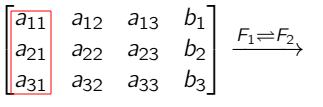
\includegraphics[scale=0.7]{Mat_pivot1.png} 
\end{center}

%$$\begin{bmatrix}
% a_{11} & a_{12} & a_{13}  &b_1\\
% a_{21} & a_{22} & a_{23} &b_2\\
% a_{31} & a_{32} & a_{33} &b_3
%
%\end{bmatrix} \xrightarrow{F_1 \rightleftharpoons F_2}  $$

\pause Esto se repetira siempre antes de cada operación principal. con los elementos restantes:

\begin{center}
	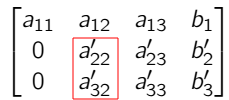
\includegraphics[scale=0.7]{Mat_pivot2.png} 
\end{center}
%$$\begin{bmatrix}
% a_{11} & a_{12} & a_{13}  &b_1\\
% 0 & a_{22}' & a_{23}' &b_2'\\
% 0 & a_{32}' & a_{33}' &b_3'
%
%\end{bmatrix} $$

\end{frame}

\subsection{Consideraciones}

\begin{frame}
\frametitle{Consideraciones}

\textbf{Consideraciones}
\pause
\begin{itemize}
\item Soluciona 0 en elemento principal.
\item Aumenta el numero de operaciones.
\item No afecta el resultado.
\item Hay que guardar los cambios de filas para recuperar el resultado original.

\end{itemize}

\end{frame}

\section{Descomposición LU}

\begin{frame}
\frametitle{Descomposición LU}

¿Debemos volver a aplicar el algoritmo si cambia mi vector b? \vspace{20pt}



Existen otros métodos.\vspace{20pt}



\pause
\begin{tcolorbox}
	\textbf{Factorización LU}
\end{tcolorbox}
\end{frame}

\begin{frame}
\frametitle{Descomposición LU}
$A = L U $ donde $L$ es triangular inferior y $ U$ es triangular superior.

Convertimos el problema:
\begin{center}
	$ A x = b $\pause $ \rightarrow L U x = b$
\end{center}

\pause
Si aplicamos el cambio de variables $ y = U x $ entonces tenemos 2 problemas 

\begin{minipage}{.45\linewidth}
\begin{equation}
 \underbrace{L y = b}_{\text{Sustitución hacia adelante}}
\end{equation}
\end{minipage}  \begin{minipage}{.45\linewidth}
\begin{equation}
\underbrace{ U x = y}_{\text{Sustitución hacia atrás}}
\end{equation} \end{minipage}

\pause
\begin{tcolorbox}
 \begin{center}
   \textbf{¿Cómo realizamos este cambio?} 
 \end{center}
\end{tcolorbox}

\end{frame}

\subsection{Matrices Elementales}

\begin{frame}
\frametitle{Matrices Elementales}
Cada operación de Gauss-Jordan puede escribirse como una matriz elemental.

$$\begin{bmatrix}
a_{11} & a_{12} & a_{13}\\
a_{21} & a_{22} & a_{23}\\
a_{31} & a_{32} & a_{33}
\end{bmatrix} \xrightarrow[F_3 - \frac{a_{31}}{a_{11}}F_1]{F_2 - \frac{a_{21}}{a_{11}}F_1}
\begin{bmatrix}
a_{11} & a_{12} & a_{13}\\
0 & a_{22}- {\color{red}\frac{a_{21}}{a_{11}}} a_{12} & a_{23}-{\color{red}\frac{a_{21}}{a_{11}}}a_{13}\\
0 & a_{32}- {\color{red}\frac{a_{31}}{a_{11}}} a_{12} & a_{33}-{\color{red}\frac{a_{31}}{a_{11}}}a_{13}
\end{bmatrix}$$


Puede expresarse cómo $E_1 A$, con 

$$E_1 =\begin{bmatrix}
1 & 0 & 0\\
-\frac{a_{21}}{a_{11}} & 1 & 0\\
-\frac{a_{31}}{a_{11}} & 0 & 1
\end{bmatrix}$$


\end{frame}

\begin{frame}
\frametitle{Matrices Elementales}
$$\begin{bmatrix}
1 & 0 & 0\\
-\frac{a_{21}}{a_{11}} & 1 & 0\\
-\frac{a_{31}}{a_{11}} & 0 & 1
\end{bmatrix}  \begin{bmatrix}
a_{11} & a_{12} & a_{13}\\
a_{21} & a_{22} & a_{23}\\
a_{31} & a_{32} & a_{33}
\end{bmatrix} = $$


$$\begin{bmatrix}
a_{11} & a_{12} & a_{13}\\
0 & a_{22}- {\color{red}\frac{a_{21}}{a_{11}}} a_{12} & a_{23}-{\color{red}\frac{a_{21}}{a_{11}}}a_{13}\\
0 & a_{32}- {\color{red}\frac{a_{31}}{a_{11}}} a_{12} & a_{33}-{\color{red}\frac{a_{31}}{a_{11}}}a_{13}
\end{bmatrix}$$
\end{frame}


\begin{frame}
\frametitle{Matrices Elementales}

\begin{itemize}
\item Son Matrices triangular inferior.
\item el producto de 2 matrices triangular inferior da otra matriz triangular inferior.
\item el producto de 2 matrices elementales no es necesariamente otra matriz elemental.
\end{itemize}
La inversa de una matriz elemental se puede calcular cambiando los signos de todos los elementos fuera de la diagonal.

$$ E_1 = \begin{bmatrix}
1 &0 & 0\\
f_{21}& 1 &0 \\
f_{31}& 0 &1 
\end{bmatrix} \rightarrow E_1^{-1} = \begin{bmatrix}
1 &0 & 0\\
{\color{red} -} f_{21}& 1 &0 \\
{\color{red} -} f_{31}& 0 &1 
\end{bmatrix}$$
\end{frame}

\subsection{Descomposición LU}
\begin{frame}
\frametitle{Descomposición LU}
Aplicar Gauss-Jordan, equivale a transformar la matriz $A$ en una matriz del tipo $U$ aplicando operaciones $E_i$:
$$ E_i * E_{i-1}* ....* E_2 * E_1 A = U $$
Si multiplicamos por la inversa de $E_i$:
$$ \underbrace{E_i^{-1} * E_i}_{I} * E_{i-1}* ....* E_2 * E_1 A = E_i^{-1} * U $$
Si realizamos esto para todas las matrices E:
$$ A = \underbrace{E_1^{-1} *E_2^{-1} *...*E_i^{-1}}_{L} * U$$

\begin{tcolorbox}
$$A = L * U $$
\end{tcolorbox}
\end{frame}

\begin{frame}
\frametitle{Descomposición LU}
En el caso de Gauss Jordan las matrices e tendrán la forma:
$E_1 = \begin{bmatrix}
1 		&0 & 0 \dots & 0 \\
f_{21} 	&1 & 0 &\dots & 0 \\
f_{31} 	&0 & 1 &\dots & 0 \\
\vdots & & &  \vdots \\
f_{n1} 	&0 & 0 \dots & 1 \\
\end{bmatrix}$, $E_2 = \begin{bmatrix}
1 &0 		& 0 &\dots & 0 \\
0 &1 		& 0 &\dots & 0 \\
0 &f_{32} 	& 1 &\dots & 0 \\
\vdots & \vdots& 	&		&  \vdots \\
0 & f_{n2} & 0 & \dots & 1 \\
\end{bmatrix}$ ....
Queda a cargo del estudiante  Probar para matrices de $4\times4$ que 
$$ E_1*E_2*E_3 = \begin{bmatrix}
1 		& 0 		& 0 		& 0\\
f_{21} 	& 1 		& 0 		& 0\\
f_{31} 	& f_{32}	& 1 		& 0\\
f_{41} 	& f_{42}	& f_{43}	& 1\\
\end{bmatrix}$$

\end{frame}

\subsection{Ejemplo LU}

\begin{frame}
\frametitle{Descomposición LU: un ejemplo}

\visible<1->{Supongamos que tenemos el problema:
$$  \begin{bmatrix}
2 & 3 & 5 \\
1 & 1 & 3 \\
3 & 2 & 3
\end{bmatrix} x = \begin{bmatrix}
10\\
5\\
8
\end{bmatrix} $$}

\begin{center}
\visible<2->{$\begin{bmatrix}
2 & 3 & 5 \\
1 & 1 & 3 \\
3 & 2 & 3
\end{bmatrix} $} \visible<3->{$\xrightarrow[F_3 -{\color{red}\frac{3}{2} }F_1]{F_2 -{\color{red}\frac{1}{2} }F_1} \begin{bmatrix}
2 & 3 & 5 \\
0 & -\frac{1}{2} & \frac{1}{2} \\
0 & -\frac{5}{2} & -\frac{9}{2}
\end{bmatrix} $} \visible<5->{$\xrightarrow{F_3 -{\color{red} 5 }F_2} \begin{bmatrix}
2 & 3 & 5 \\
0 & -\frac{1}{2} & \frac{1}{2} \\
0 &  0 & -7
\end{bmatrix} $}
\end{center}


\begin{center}
\visible<4->{$E_1^{-1} = \begin{bmatrix}
1 			& 0 & 0 \\
\frac{1}{2} 	& 1 & 0 \\
\frac{3}{2} 	& 0 & 1 
\end{bmatrix}$,} \visible<6->{$E_2^{-1} = \begin{bmatrix}
1 			& 0 & 0 \\
0		 	& 1 & 0 \\
0		 	& 5 & 1 
\end{bmatrix}$}
\end{center}

\end{frame}



\begin{frame}
\frametitle{Descomposición LU: un ejemplo}
$$ U = \begin{bmatrix}
2 & 3 & 5 \\
0 & -\frac{1}{2} & \frac{1}{2} \\
0 &  0 & -7
\end{bmatrix}$$
\pause
$$L = E_1^{-1} * E_2^{-1} = \begin{bmatrix}
1 			& 0 & 0 \\
\frac{1}{2} 	& 1 & 0 \\
\frac{3}{2} 	& 0 & 1 
\end{bmatrix} \begin{bmatrix}
1 			& 0 & 0 \\
0		 	& 1 & 0 \\
0		 	& 5 & 1 
\end{bmatrix} = \underbrace{\begin{bmatrix}
1 			& 0 & 0 \\
\frac{1}{2} 	& 1 & 0 \\
\frac{3}{2} 	& 5 & 1 
\end{bmatrix}}_{L}$$
\pause
Veamos que $L*U = A$

$$\begin{bmatrix}
1 			& 0 & 0 \\
\frac{1}{2} 	& 1 & 0 \\
\frac{3}{2} 	& 5 & 1 
\end{bmatrix} \begin{bmatrix}
2 & 3 & 5 \\
0 & -\frac{1}{2} & \frac{1}{2} \\
0 &  0 & -7
\end{bmatrix} = \begin{bmatrix}
2 & 3 & 5\\
1 & 1 & 3\\
3 & 2 & 3
\end{bmatrix}  $$

\end{frame}


\begin{frame}
\frametitle{Descomposición LU: un ejemplo}
Ahora son 2 problemas:

\begin{minipage}{.45\linewidth}
\begin{equation}\label{eq:y}
L y = b
\end{equation}
\end{minipage}  \begin{minipage}{.45\linewidth}
\begin{equation}\label{eq:x}
U x = y
\end{equation}
\end{minipage}
\pause

Para la ec. \ref{eq:y}
$$\begin{bmatrix}
1 			& 0 & 0 \\
\frac{1}{2} 	& 1 & 0 \\
\frac{3}{2} 	& 5 & 1 
\end{bmatrix} y = \begin{bmatrix}
10\\ 
5\\
8
\end{bmatrix} $$

\begin{minipage}{.6\linewidth}
\pause

$y_1 = 10$ ,\pause $y_2 +\frac{1}{2} y_1 = 5$ \pause $\rightarrow y_2 = 0$, \pause 

$y_3 +\frac{3}{2} y_1 + 5 y_2 = 8 \rightarrow y_3 =-7$ 

\end{minipage} \vline  \begin{minipage}{.3\linewidth}
$$\boxed{y = \begin{bmatrix}
10\\
0\\
-7
\end{bmatrix} }$$
\end{minipage}

\end{frame}


\begin{frame}
\frametitle{Descomposición LU: un ejemplo}
Para la ec. \ref{eq:x}

$$\begin{bmatrix}
2 			& 3 				& 5 \\
0			& -\frac{1}{2} 	& \frac{1}{2} \\
0		 	& 0 				& -7 
\end{bmatrix} x = \begin{bmatrix}
10\\ 
0\\
-7
\end{bmatrix} $$

\begin{minipage}{.6\linewidth}
\pause

$x_3 = 1$ ,\pause $-\frac{1}{2} x_2 +\frac{1}{2} x_3 = 0$ \pause $\rightarrow x_2 = 1$, \pause 

$2 x_1 +3 x_2 + 5 x_3 = 10 \rightarrow x_1 =1$ 

\end{minipage} \vline  \begin{minipage}{.3\linewidth}
$$\boxed{x = \begin{bmatrix}
1\\
1\\
1
\end{bmatrix} }$$
\end{minipage}

\end{frame}



\end{document}

%%% Local Variables: 
%%% mode: latex
%%% TeX-master: t
%%% End: 







